\documentclass[12pt, oneside]{article}

% Language setting
% Replace `english' with e.g. `spanish' to change the document language
\usepackage[english]{babel}

% Set page size and margins
% Replace `letterpaper' with `a4paper' for UK/EU standard size
\usepackage[letterpaper,top=2cm,bottom=2cm,left=3cm,right=3cm,marginparwidth=1.75cm]{geometry}

% Useful packages
\usepackage{amsmath}
\usepackage{graphicx}
\usepackage[colorlinks=true, allcolors=blue]{hyperref}
\usepackage{graphicx} % Required for inserting images
\usepackage{cite}
\usepackage{amsmath,amssymb,amsfonts}
\usepackage{algorithmic}
\usepackage{graphicx}
\usepackage{textcomp}
\usepackage{xcolor}
\usepackage{csquotes}
\usepackage{placeins}
\usepackage{etoolbox}
\usepackage{graphicx}
\usepackage{wrapfig}
\usepackage{subfigure}
\usepackage{subcaption}
\usepackage{IEEEtrantools}

\begin{document}

\begin{titlepage}
    \begin{center}
        \vspace*{1cm}
        {\huges
        \center{\huge{\textbf{Advanced Control and Dynamics}}}}
         \\
         \vspace{0.3cm}
         \large{Coursework Report}
         \vspace{0.5cm}
        \\
        {\large By}
        \\
        \vspace{0.5cm}
        \textbf{Runze Yuan}
        \\
        \vspace{0.5cm}
        Student Number: 22071714
   		\vspace{1.5cm}
        \\
        \vspace{0.25cm}
       
\includegraphics[scale=0.6]{logos/bristolcrest_colour.pdf}
        \hspace{5mm}
        
\includegraphics[scale=0.35]{logos/UWE_insignia.png}

        \vspace{10mm}
        {\large Department of Engineering Mathematics\\
        \textsc{University of Bristol}}
        \\
        \&
        \\
        {\large Department of Engineering Design and Mathematics\\
        \textsc{University of the West of England}}\\

        \vspace{0.8cm}
 
        \vspace{0.8cm}
        \today
        
    \end{center}
    
\end{titlepage}

\tableofcontents
\pagebreak

\section{Practical Plant Definition}

% http://sim.okawa-denshi.jp/en/CRCRkeisan.htm


\textbf{Question:} 
\begin{quote}
Define a practical engineering plant which would feature similar dynamical behaviour to the theoretical dynamics given in the plant description below. Briefly describe the operation of the plant.
\end{quote}

Theoretical transfer function of the plant:

\begin{equation}
    \frac{Y(s)}{U(s)} = g_{p}(s) = \frac{1}{s^{2}+0.6s+4}
\end{equation}
\textbf{Answer:}
% https://electronics.stackexchange.com/questions/152159/deriving-2nd-order-passive-low-pass-filter-cutoff-frequency
\vspace{0.5cm}


\begin{figure}[htbp]
  \begin{minipage}[t]{0.5\textwidth}
    \centering
    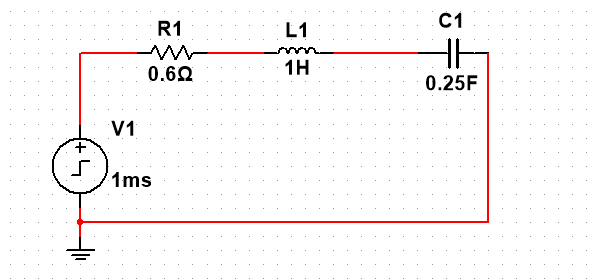
\includegraphics[width=\linewidth]{Report/pics/RLC电路例子.png}
    \caption{Example of RLC circuit. 
    \centering
    \begin{Large}
    $\frac{U_c}{V_1} = \frac{4}{s^2+0.6s+4}$.
    \end{Large}
    }
    \label{fig:RLC circuit example}
  \end{minipage}
  \hfill
  \begin{minipage}[t]{0.5\textwidth}
    \centering
    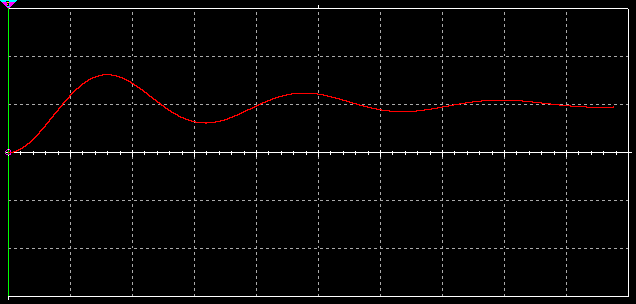
\includegraphics[width=\linewidth]{Report/pics/RLCStepResponse.png}
    \caption{Simulated step response of voltage across capacitor C1. }
    \label{fig:Uc step response}
  \end{minipage}
\end{figure}

A common example which has similar dynamic with the given transfer function is a RLC circuit.

As shown in Fig. \ref{fig:RLC circuit example}, the voltage across the capacitor C1 exhibits dynamic characteristics similar to the given transfer function. Explains are as follows:

\vspace{0.2cm}
Voltage equation of the entire circuit in time domain:
\begin{equation}
    V_1 = U_R+U_L+U_C = R\times I+L\times \frac{dI}{dt}+\frac{1}{C}\int_0^t Idt
    \label{equ:VoltageInTimeDomain}
\end{equation}

Apply Laplacian transform on equation (\ref{equ:VoltageInTimeDomain}), and we have:
\begin{equation}
        V_1(s) = RI(s)+ LI(s)s+\frac{I(s)}{Cs}
        \label{equ:VoltageInSDomain}
\end{equation}

And from equation (\ref{equ:VoltageInSDomain}), the relation of voltage across the capacitor and the source is:
\begin{equation}
    \frac{U_C(s)}{V_1(s)}=\frac{1}{LCs^2+CRs+1}
\end{equation}

Which have similar dynamic with the theoretical plant provided. The simulated step response of voltage across capacitor C1 is shown in Fig. \ref{fig:Uc step response}.

\pagebreak

\section{Control System Block Diagrams}
\textbf{Question:}
\begin{quote}
    Draw two equivalent control system block diagrams, which features the output feedback and the state feedback respectively. Compare the similarity and difference. 
\end{quote}
\textbf{Answer:}

\begin{figure}[htbp]
    \centering
    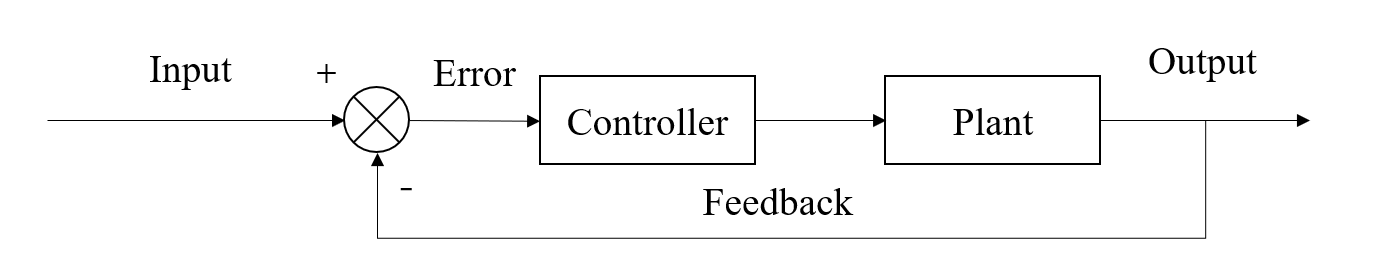
\includegraphics[height = 0.07\paperheight]{Report/pics/OutputFeedbackDiagram.png}
    \caption{Output feedback control diagram.}
    \label{fig:my_label}
\end{figure}

\begin{figure}[htbp]
    \centering
    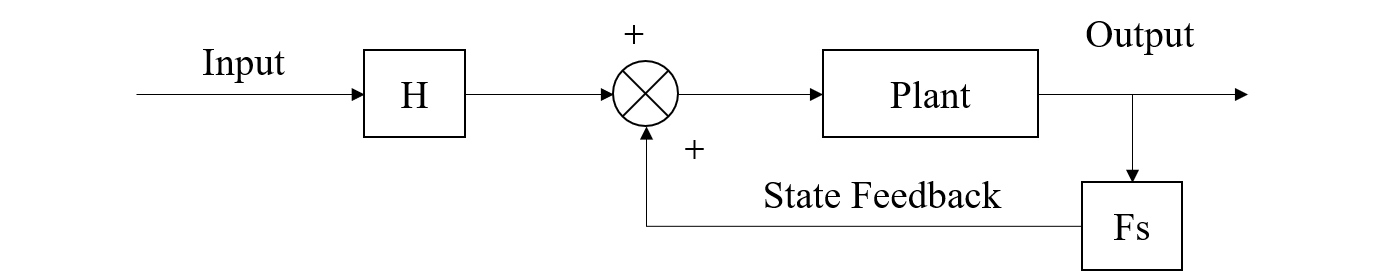
\includegraphics[height = 0.1\paperheight]{Report/pics/StateFeedbackDiagram.png}
    \caption{State feedback control diagram.}
    \label{fig:my_label}
\end{figure}


\textbf{Similarity}
\begin{itemize}
    \item Both methods are used to modify the performance of the system to achieve the desired outcome.
    \item Both methods are close loop control and using feedback to accomplish the objective of control.
    \item Both require the mathematical model of the system.
    \item Both methods using linear controlling techniques like poles placing, etc.
\end{itemize}

\textbf{Difference}
\begin{itemize}
    \item State feedback cannot apply to systems whose states are not observable, while the output feedback requires the output only.
    \item The core idea is different: output feedback aims to eliminate/minimize errors, but state feedback is about changing the plant characteristics and creating an ideal system which including the plant as a subsystem.
    \item Output feedback is actually a kind of partially state feedback, for output is a combination of the states. But not all states could be found in output, so the freedom of output feedback is lesser than state feedback.
    \item Output feedback is more suitable for systems that are uncertain and have disturbance.
    \item State feedback is more suitable for systems that are fully examined and have less disturbance.
\end{itemize}



\section{Plant Analyse}

\textbf{Question:}

\begin{quote}    
Analyse the plant performance such stability, observability, controllability, and time response to a unit step reference input.
\end{quote}
\textbf{Answer:}
\begin{itemize}
    \item \textbf{Stability:}
    Poles of the plant are: $-0.3000\pm1.9774i$, both of them are on the left-half of the s-plane, which means that the system is stable.
    \item \textbf{Observability and controllability:} For linear time-invariant systems, controllability and observability are equivalent in continuous time. The following verification is using the observable realisation:

    \begin{equation}
        \begin{cases}
        \left[\begin{array}{ccc}\dot{x_1}(t)\\
        \dot{x_{2}}(t)\end{array}\right]
        =
        \left[\begin{array}{ccc} 0&-4\\
        1&-0.6\end{array}\right]
        \left[\begin{array}{ccc}x_1(t)\\
        x_2(t)\end{array}\right]
        +
        \left[\begin{array}{ccc}1\\
        0\end{array}\right]
        u(t)
        \\
        \\
        y(t)=
        \left[\begin{array}{ccc}1&0\end{array}\right]
        \left[\begin{array}{ccc}x_1(t)\\
        x_2(t)\end{array}\right]
        \end{cases}
    \end{equation}

    For the realisation above, the criterion matrices P, Q and R are:
    $P = \left[\begin{array}{ccc}1&0\\
        0&1\end{array}\right]$, $Q = \left[\begin{array}{ccc}0&1\end{array}\right]$, $R=\left[\begin{array}{ccc}0&1\\
        1&-0.6\end{array}\right]$. It's controllable ($rank(P)=2=n, rank(Q)=1=l$) and observable ($rank(R)=2=n$).

    
    \item \textbf{Unit step response:} The unit step response in time domain is as shown in Fig. \ref{fig:PlantStepResponse}. This plant has a slow response speed and steady-state error.


        \begin{figure}[htbp]
          \centering
          \subfigure[Simulated step response in Simulink.\label{fig:PlantStepResponse}]{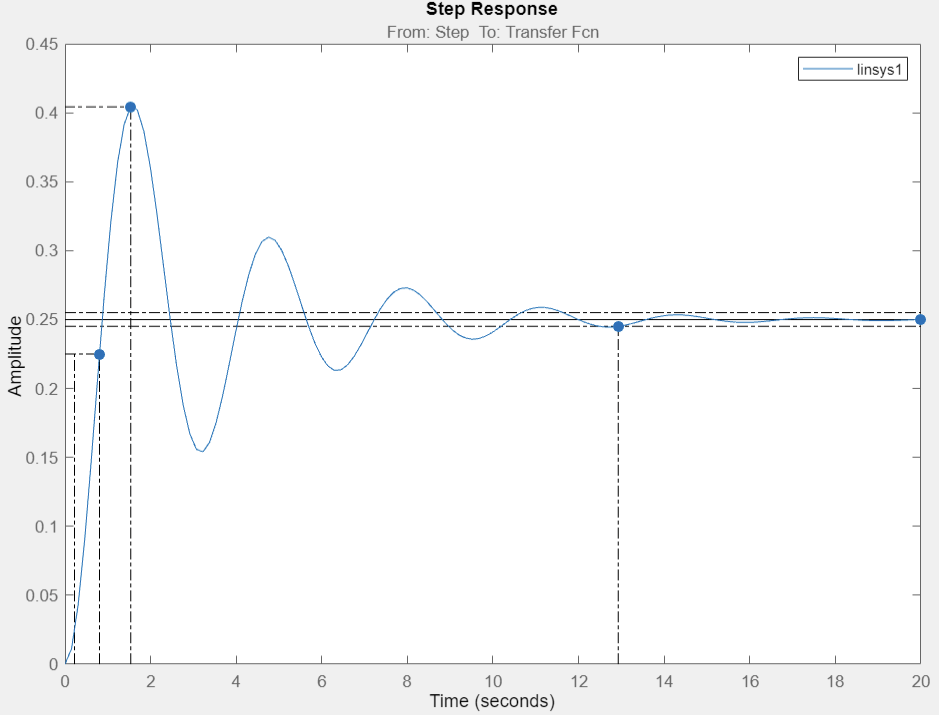
\includegraphics[width=0.45\textwidth]{Report/pics/PlantStepResponse.png}}
          \quad % or \hfill
          \subfigure[Simulated step response in MATLAB.\label{fig:SimulatedStepResponse} ]{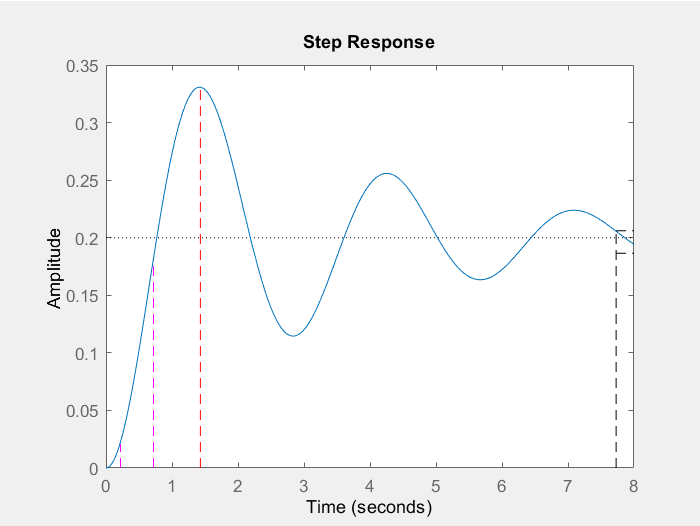
\includegraphics[width=0.45\textwidth]{Report/pics/SimulateStepResponse.png}}
          \caption{Simulated step responses.}
        \end{figure}

    \item \textbf{Other Metrics:}  Other common metrics for second order system performance evaluation:
        \begin{itemize}
            \item Overshoot: 68.4885\%
            \item Steady-state error: 0.80372
            \item Rise time: 0.5 s
            \item Peak time: 1.43 s
            \item Settling time: 7.73 s (error$\leq$ 5\%)
        \end{itemize}
\end{itemize}



\section{State Feedback Controller Design}
\textbf{Question:}
\begin{quote}
Design a state feedback controller (you specify the reasonable design criteria).
\end{quote}
\textbf{Answer:}

 \textbf{Damping ratio $\xi$ :} Choose the optimal damping ratio $\xi=0.707$. The optimal damping ratio can minimize the cumulative error and its rate of change.
 
 \textbf{Undamped natural frequency $\omega_n$:} Assuming we need to achieve a settling time (5\% error) of 0.5 seconds, the natural frequency of oscillation would be: $\omega_n = 0.5\times\frac{\xi}{3}=6\sqrt{2}.$

 \textbf{Closed loop denominator}: $s^2+2\xi\omega_{n}s+\omega_{n}^2 \rightarrow s^2+12s+72$.

 From the closed loop denominator and steady state final value, we have:
 \begin{equation}
     \begin{cases}
         F_s = \left[\begin{array}{ccc}-\frac{57}{5}&-\frac{1529}{25}\end{array}\right]\approx\left[\begin{array}{ccc}-11.4&-61.16\end{array}\right]\\
         H=100
     \end{cases}
 \end{equation}

And the closed loop state feedback controller is as shown below:
 \begin{figure}[htbp]
     \centering
     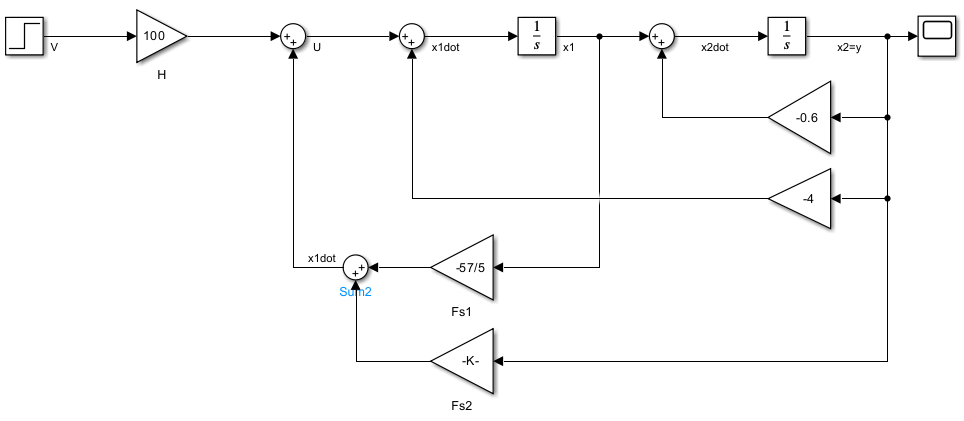
\includegraphics[width = 0.9\textwidth]{Report/pics/StateFeedbackControl.png}
     \caption{Plant with state feedback control.}
     \label{fig:State Feedback Control}
 \end{figure}
\FloatBarrier
 

\section{Observer Design}


\section{Performance Simulation}
\section{Digital Controller Implementation}
\section{References}

\end{document}